\documentclass{article}
\usepackage[utf8]{inputenc}
\usepackage[section]{placeins}
\usepackage{graphicx}
\graphicspath{{./images/}}
\usepackage{float}

\usepackage{titlesec}
\newcommand{\sectionbreak}{\clearpage} %makes it so sections start new pages.

\title{jRAPL Runtime Data Collection}
\author{Alejandro Servetto, Rutvik Saptarshi}
\date{April 2020}

\begin{document}

\maketitle

\section{Introduction}
This document contains graphs from runtime tests of existing jRAPL functions on Rutvik's Acer Nitro and Alejandro's Lenovo Ideapad.

Graphs below include comparison of run time of functions between C and Java, scatter plots that show the distribution and outliers of runtime in the C functions, comparing the time it takes to read an MSR register per power domain, AND OTHER STUFF TOO THAT I SHOULD MAKE SURE I INCLUDED

\section{System Specs}
Experiments are run on two computers, System A and System B.

\textbf{Specs for System A:}
\begin{itemize}
    \item Name: Lenovo Ideapad 120s-11IAP
    \item CPU: Intel Celeron N3350 / 1.1 GHz
    \item GPU: 
    \item RAM: 2GB LPDDR4 SDRAM
    \item OS: Linux Mint Cinnamon 19.1
    \item Linux Kernel Version: 4.15.0-20-generic
\end{itemize}
    
\textbf{Specs for System B:}
\begin{itemize}
    \item Name: Acer Nitro
    \item CPU: Intel Core i5-9300H @ 2.40 GHz quadcore
    \item GPU: NVIDIA GTX 1650 4GB graphics memory GDDR5
    \item RAM: 8GB DDR4 SDRAM
    \item OS: Ubuntu 12.04.4 LTS
    \item Linux Kernel Version: 5.3.0-46-generic
\end{itemize}


\section{Comparing C and Java Runtime}
This section is dedicated to showing the overhead that calling C functions via the Java native interface adds. To do this, we timed the Java functions, as well as internally timing the C functions. Each side of function calling received 4000 consecutive trials, and then we compared averages and standard deviations per function.


\section{Scatter Plots of C Function Runtime}
The graphs below show the runtime of each individual C function run. The purpose of these graphs is to show the distribution of C runtimes and how the results usually cluster around a certain value, but some outliers drastically skew the average and standard deviation. The most notable example is the ProfileInit() function, which has most values in the low 2 digits, but has a few in the tens of thousands.\\

\textbf{C Runtimes on System A}
\begin{figure}[H]
	\centering
	\includegraphics[width=10cm,height=10cm,keepaspectratio]{RuntimeResults_SystemA/CFunctions/ProfileDealloc_scatter.png}
	\caption{Scatter plot of C-Functions runtime for ProfileDealloc for SystemA}
	\label{fig:C-Functions|ProfileDealloc|SystemA}
\end{figure}

\begin{figure}[H]
	\centering
	\includegraphics[width=10cm,height=10cm,keepaspectratio]{RuntimeResults_SystemA/CFunctions/ProfileInit_scatter.png}
	\caption{Scatter plot of C-Functions runtime for ProfileInit for SystemA}
	\label{fig:C-Functions|ProfileInit|SystemA}
\end{figure}

\begin{figure}[H]
	\centering
	\includegraphics[width=10cm,height=10cm,keepaspectratio]{RuntimeResults_SystemA/CFunctions/EnergyStatCheck_scatter.png}
	\caption{Scatter plot of C-Functions runtime for EnergyStatCheck for SystemA}
	\label{fig:C-Functions|EnergyStatCheck|SystemA}
\end{figure}

\begin{figure}[H]
	\centering
	\includegraphics[width=10cm,height=10cm,keepaspectratio]{RuntimeResults_SystemA/CFunctions/GetSocketNum_scatter.png}
	\caption{Scatter plot of C-Functions runtime for GetSocketNum for SystemA}
	\label{fig:C-Functions|GetSocketNum|SystemA}
\end{figure}

\textbf{C Runtimes on System B}

\begin{figure}[H]
	\centering
	\includegraphics[width=10cm,height=10cm,keepaspectratio]{RuntimeResults_SystemB/CFunctions/ProfileDealloc_scatter.png}
	\caption{Scatter plot of C-Functions runtime for ProfileDealloc for SystemB}
	\label{fig:C-Functions|ProfileDealloc|SystemB}
\end{figure}

\begin{figure}[H]
	\centering
	\includegraphics[width=10cm,height=10cm,keepaspectratio]{RuntimeResults_SystemB/CFunctions/ProfileInit_scatter.png}
	\caption{Scatter plot of C-Functions runtime for ProfileInit for SystemB}
	\label{fig:C-Functions|ProfileInit|SystemB}
\end{figure}

\begin{figure}[H]
	\centering
	\includegraphics[width=10cm,height=10cm,keepaspectratio]{RuntimeResults_SystemB/CFunctions/EnergyStatCheck_scatter.png}
	\caption{Scatter plot of C-Functions runtime for EnergyStatCheck for SystemB}
	\label{fig:C-Functions|EnergyStatCheck|SystemB}
\end{figure}

\begin{figure}[H]
	\centering
	\includegraphics[width=10cm,height=10cm,keepaspectratio]{RuntimeResults_SystemB/CFunctions/GetSocketNum_scatter.png}
	\caption{Scatter plot of C-Functions runtime for GetSocketNum for SystemB}
	\label{fig:C-Functions|GetSocketNum|SystemB}
\end{figure}



\section{Scatter Plots of Java Function Runtime}
The graphs below show the runtime of each individual Java function run. The purpose of these graphs is to show the distribution of Java runtimes and how the results usually cluster around a certain value, but some outliers drastically skew the average and standard deviation. The most notable example is the ProfileInit() function, which has most values in the low 2 digits, but has a few in the tens of thousands.\\

\textbf{Java Runtimes on System A}

\begin{figure}[H]
	\centering
	\includegraphics[width=10cm,height=10cm,keepaspectratio]{RuntimeResults_SystemA/JavaFunctions/ProfileDealloc_scatter.png}
	\caption{Scatter plot of Java-Functions runtime for ProfileDealloc for SystemA}
	\label{fig:Java-Functions|ProfileDealloc|SystemA}
\end{figure}

\begin{figure}[H]
	\centering
	\includegraphics[width=10cm,height=10cm,keepaspectratio]{RuntimeResults_SystemA/JavaFunctions/ProfileInit_scatter.png}
	\caption{Scatter plot of Java-Functions runtime for ProfileInit for SystemA}
	\label{fig:Java-Functions|ProfileInit|SystemA}
\end{figure}

\begin{figure}[H]
	\centering
	\includegraphics[width=10cm,height=10cm,keepaspectratio]{RuntimeResults_SystemA/JavaFunctions/EnergyStatCheck_scatter.png}
	\caption{Scatter plot of Java-Functions runtime for EnergyStatCheck for SystemA}
	\label{fig:Java-Functions|EnergyStatCheck|SystemA}
\end{figure}

\begin{figure}[H]
	\centering
	\includegraphics[width=10cm,height=10cm,keepaspectratio]{RuntimeResults_SystemA/JavaFunctions/GetSocketNum_scatter.png}
	\caption{Scatter plot of Java-Functions runtime for GetSocketNum for SystemA}
	\label{fig:Java-Functions|GetSocketNum|SystemA}
\end{figure}

\textbf{Java Runtimes on System B}

\begin{figure}[H]
	\centering
	\includegraphics[width=10cm,height=10cm,keepaspectratio]{RuntimeResults_SystemB/JavaFunctions/ProfileDealloc_scatter.png}
	\caption{Scatter plot of Java-Functions runtime for ProfileDealloc for SystemB}
	\label{fig:Java-Functions|ProfileDealloc|SystemB}
\end{figure}

\begin{figure}[H]
	\centering
	\includegraphics[width=10cm,height=10cm,keepaspectratio]{RuntimeResults_SystemB/JavaFunctions/ProfileInit_scatter.png}
	\caption{Scatter plot of Java-Functions runtime for ProfileInit for SystemB}
	\label{fig:Java-Functions|ProfileInit|SystemB}
\end{figure}

\begin{figure}[H]
	\centering
	\includegraphics[width=10cm,height=10cm,keepaspectratio]{RuntimeResults_SystemB/JavaFunctions/EnergyStatCheck_scatter.png}
	\caption{Scatter plot of Java-Functions runtime for EnergyStatCheck for SystemB}
	\label{fig:Java-Functions|EnergyStatCheck|SystemB}
\end{figure}

\begin{figure}[H]
	\centering
	\includegraphics[width=10cm,height=10cm,keepaspectratio]{RuntimeResults_SystemB/JavaFunctions/GetSocketNum_scatter.png}
	\caption{Scatter plot of Java-Functions runtime for GetSocketNum for SystemB}
	\label{fig:Java-Functions|GetSocketNum|SystemB}
\end{figure}

\section{Per Socket MSR Reading}
jRAPL currently reads from 4 MSRs that store total system energy consumption for 4 power domains: Package, CPU, DRAM, and GPU. However, individual computer models only provide readings for either DRAM or GPU. Our computers only have one socket and both read energy from DRAM, not GPU
%Below are graphs comparing the runtime of reading each MSR for our computers.

\begin{figure}[H]
	\centering
	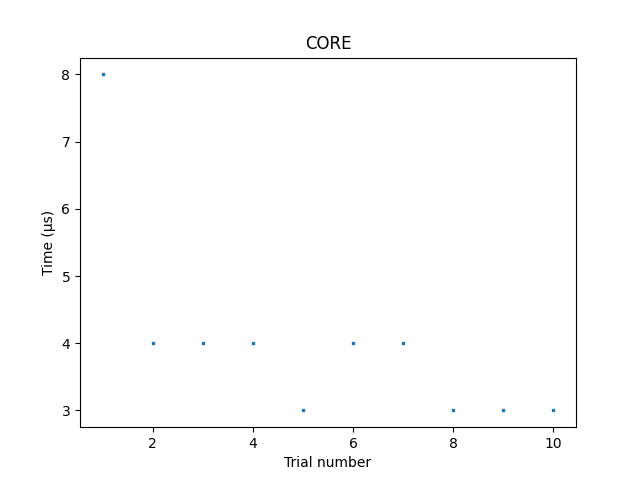
\includegraphics[width=10cm,height=10cm,keepaspectratio]{RuntimeResults_SystemB/PerSocketMSRReadings/Socket0/CORE_scatter.png}
	\caption{Scatter plot of Per-Socket-MSR-Readings runtime for CORE for SystemB}
	\label{fig:Per-Socket-MSR-Readings|CORE|SystemB}
\end{figure}

\begin{figure}[H]
	\centering
	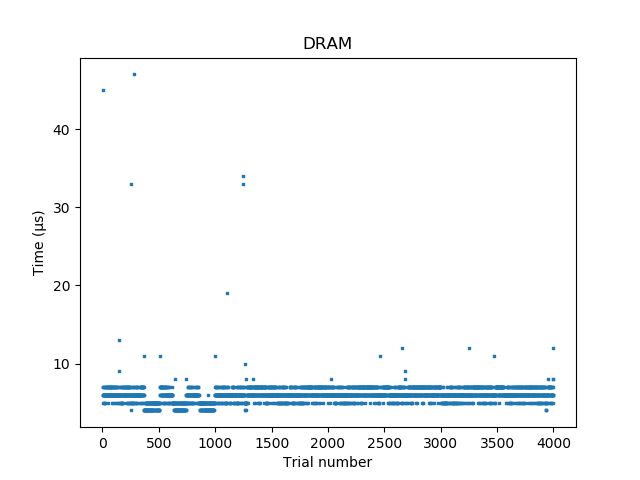
\includegraphics[width=10cm,height=10cm,keepaspectratio]{RuntimeResults_SystemB/PerSocketMSRReadings/Socket0/DRAM_scatter.png}
	\caption{Scatter plot of Per-Socket-MSR-Readings runtime for DRAM for SystemB}
	\label{fig:Per-Socket-MSR-Readings|DRAM|SystemB}
\end{figure}

\begin{figure}[H]
	\centering
	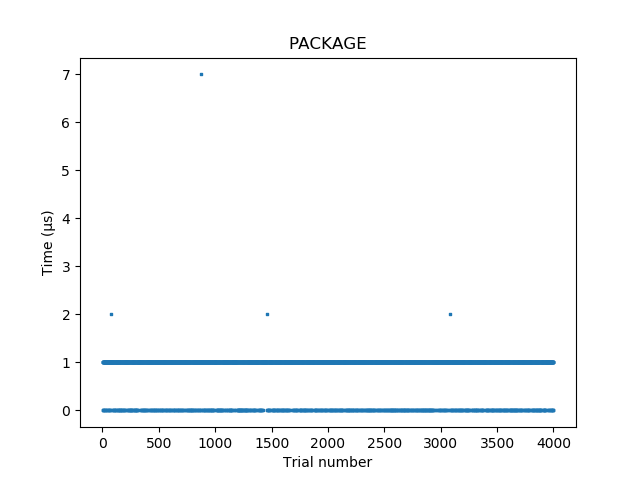
\includegraphics[width=10cm,height=10cm,keepaspectratio]{RuntimeResults_SystemB/PerSocketMSRReadings/Socket0/PACKAGE_scatter.png}
	\caption{Scatter plot of Per-Socket-MSR-Readings runtime for PACKAGE for SystemB}
	\label{fig:Per-Socket-MSR-Readings|PACKAGE|SystemB}
\end{figure}

\begin{figure}[H]
	\centering
	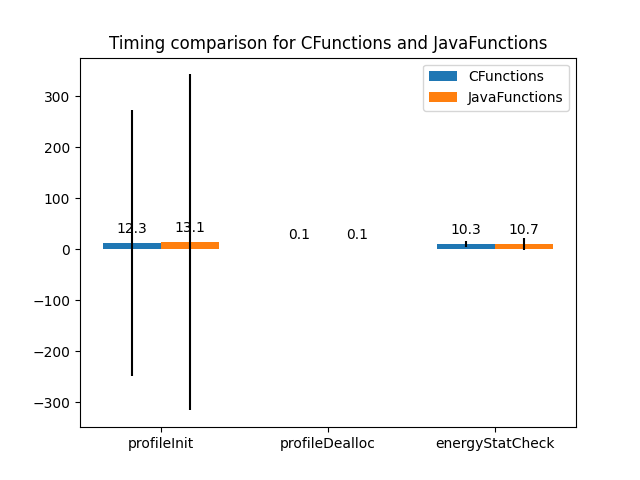
\includegraphics[width=10cm,height=10cm,keepaspectratio]{RuntimeResults_SystemB/CFunctions-JavaFunctions-bar_graph.png}
	\caption{Bar graph comparing Java and C function runtime}
	\label{fig:bar-graph||SystemB}
\end{figure}


%\section{Collecting Data after CPU and Memory Stressing}
%These graphs are the result of a few data collections, measured under different CPU stress conditions (Rutvik, please explain in detail what each thing is and what means, since I only sort of get it...). Each set of data was collected on the DRAM, CPU, and Package MSR readings.

%We used the stress-ng program to put stress on the CPU, VM, and both at the same time. System A only supported 2 CPU and VM hogs to be able to complete the tasks, while System B used 4 CPU hogs and 8 VM hogs. (Should probably explain what exactly hogs are...)

%There were 72 graphs generated in total for these readings so I don't know how we're going to get them on this document...

\end{document}
